Esta seção do trabalho apresenta termos e conceitos de importância para a realização do experimento. O trabalho abrange conceitos sobre as metodologias ágeis de desenvolvimento e sobre o modelo toyotista de produção com o nome de \textit{Lean}.

\subsection{Métodos ágeis}

Desenvolvimento ágil é o termo utilizado para representar um conjunto de métodos e práticas adotados para desenvolver e entregar \textit{software} de forma rápida e incremental. As metodologias ágeis são derivadas dos valores e princípios contidos no Manifesto Ágil \cite{Manifesto}. As metodologias de desenvolvimento que surgiram a partir do Manifesto são diversas, sendo as mais populares \textit{Scrum e Extreme Programming} (XP) \cite{poth2019lean}. Nas metodologias de desenvolvimento ágil, pode-se observar semelhanças como a organização em equipes pequenas, menor hierarquização e burocratização, ciclos curtos, iterativos e incrementais de entrega e o foco na geração rápida de valor \cite{wei2019}. Com base nos fatores de sucesso observados na utilização de métodos ágeis pela indústria, acredita-se que seu uso no ensino acadêmico também possa ser bem sucedido \cite{fernandes2019identifying}.

\subsection{Metodologia \textit{Lean} e derivados}

O processo do \textit{Lean Learning} -- que será explicado mais a frente nesta seção --, possui três fases, sendo denominadas \textit{``Build, Measure e Learn"} ou ``Construir, Medir e Aprender", representadas pelos círculos azuis na Figura 1. Já os círculos verdes representam os artefatos gerados após cada fase. Após a etapa de aprender, ideias de como melhorar o ensino surgem. Depois da fase de construir, geram-se protótipos de atividades práticas para fixar o conteúdo lecionado. Após a fase de medir, dados aparecem em forma de métricas a serem avaliadas e, após essa avaliação, repete-se o ciclo em busca da melhoria contínua do aprendizado. Novamente é necessário aprender como melhorar o ensino, construir novas formas de lecionar e medir os resultados obtidos no ciclo.

\begin{figure}[!h]
    \centering
    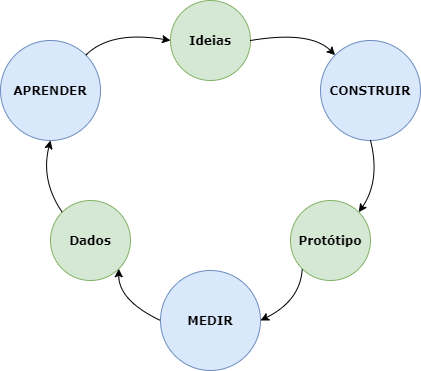
\includegraphics[width=7cm,height=5.9cm]{Imagens/Lean.png}
    \caption{Processo \textit{Lean Learning}. Fonte: autores}
    \label{fig:Processo}
\end{figure}

O \textit{Lean} visa a constante otimização dos processos produtivos e a qualidade do produto entregue. Os frutos desse modo de pensar promovem menor desperdício de recursos, redução de custos, aumento de velocidade de produção e geração de valor para o cliente. Além desses benefícios para o negócio, ele também acarreta numa harmonização maior para a equipe que, com melhores resultados, fica mais satisfeita com seu trabalho \cite{poth2019lean}.

O \textit{Lean} possui três palavras (em japonês) essenciais sobre os seus valores, sendo elas: (i) \textit{Mura}, (ii) \textit{Muri} e (iii) \textit{Muda}. \textit{Mura} significa evitar qualquer processo ou prática que não seja estável. \textit{Muri} significa evitar tarefas que possam sobrecarregar processos, pessoas e equipamentos. E \textit{Muda} significa eliminar atividades e processos identificados como inúteis e que estejam dificultando o gargalo das atividades.

O \textit{Lean Learning} consiste no uso do \textit{Lean} voltado à educação. Assim como na forma de ensino comum nas escolas e universidades, o \textit{Lean Learning} possui seus papéis \cite{chatley2017lean}. Há o papel do professor, conhecido como especialista, há o estudante e, por último, há o papel de líder. O especialista é quem leciona as disciplinas propostas e auxilia os alunos a entender o conteúdo. Os estudantes, por sua vez, serão os aprendizes do professor e realizam tarefas propostas e são avaliados pelo desempenho obtido nas atividades. O líder pode ser a mesma pessoa do professor -- seu papel é assegurar suporte institucional para o método ser devidamente aplicado. Além disso, ele incentiva uma presença mais ativa dos professores e dos demais funcionários do ambiente \cite{madruga2018}.

O processo se inicia na fase de aprender, onde é definido o que se quer aprender. Na abordagem de Boufleur et al. (2016) sobre o \textit{Lean Learning}, busca-se descobrir práticas redundantes e que não estão diretamente ligadas ao ensino. Anotação da teoria do conteúdo, inicialização a um novo tema na disciplina, atividades como estas não são focadas propriamente no aprendizado dos alunos sobre determinado assunto, mas no registro deste. Nessa fase geram-se ideias, que seriam o artefato de um cronograma de aulas, onde o professor define o que ele irá lecionar ao longo do período, quando as atividades práticas e provas irão ocorrer, quando revisar matérias entre outras atividades.

Após a fase de aprender, deve-se realizar a fase de construir, na qual é feito um novo projeto educacional visando a maior satisfação dos alunos. Como o \textit{Lean Learning} foca em atividades práticas para se fixar o conteúdo da disciplina com os alunos, nessa fase de construir geram-se os protótipos. Essas são as ideias das atividades práticas aplicadas aos alunos. Define-se o porque essa prática pode ser útil aos alunos e a qual parte da matéria lecionada ela se relaciona \cite{LeanStartup2016}. Um exemplo comum na Engenharia de \textit{Software} é a prática de montagem de aviões de papel, simulando uma rotina de trabalho em equipe com a metodologia \textit{Scrum} em uma empresa.

Por último, na fase de medir, são analisados os \textit{feedbacks} dados pelos estudantes e aplica-se o que achar necessário em busca de melhorias no ensino, seja em questão de gastos, tempo ou no desempenho dos alunos. Ao medir determinadas métricas de eficiência, dados são gerados. Esses dados informam ao professor se determinada prática foi útil ou não aos alunos, e permite ao professor retornar à fase de aprender sabendo qual atividade prática deve ser reaproveitada em outro período, e qual seria necessário ser reformulada para se tirar maior proveito dela. A etapa de medir utiliza das atividades práticas para gerar os dados que são analisados e servem como \textit{feedback} para o professor.

O \textit{Lean Learning} é um processo repetitivo, onde em cada ciclo se busca uma melhoria contínua, como visto na Figura 1. Portanto, ao acabar a fase de construir, é necessário novamente buscar possíveis novos gargalos ou atividades negativas no novo método educacional, a fim de otimizá-lo novamente \cite{LeanStartup2016}. Alguns dos artefatos produzidos ao se utilizar o processo do \textit{Lean Learning} são: ementa da disciplina, escopo de atividades práticas, provas, cronograma de aulas, trabalhos realizados, apresentações gravadas e artigos escritos.